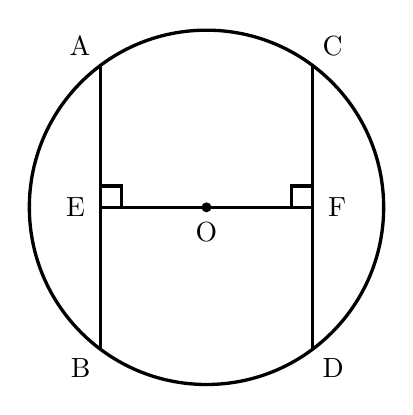
\begin{tikzpicture}[scale=1.5]
    % Draw the circle
    \draw[very thick] (0,0) circle (1.5cm);
    
    % Center point O
    \fill (0,0) circle (1.2pt);
    \node[below=2pt] at (0,0) {O};
    
    % Points A and B on the left chord (vertical)
    \coordinate (A) at (-0.9,1.2);
    \coordinate (B) at (-0.9,-1.2);
    
    % Points C and D on the right chord (vertical)
    \coordinate (C) at (0.9,1.2);
    \coordinate (D) at (0.9,-1.2);
    
    % Points E and F where horizontal line meets the chords
    \coordinate (E) at (-0.9,0);
    \coordinate (F) at (0.9,0);
    
    % Draw the two vertical chords AB and CD
    \draw[very thick] (A) -- (B);
    \draw[very thick] (C) -- (D);
    
    % Draw horizontal line EF through center
    \draw[very thick] (E) -- (F);
    
    % Right angle mark at E (upper)
    \draw[very thick] (-0.9,0.18) -- (-0.72,0.18) -- (-0.72,0);
    
    % Right angle mark at F (upper)
    \draw[very thick] (0.9,0.18) -- (0.72,0.18) -- (0.72,0);
    
    % Labels
    \node[above left] at (A) {A};
    \node[below left] at (B) {B};
    \node[above right] at (C) {C};
    \node[below right] at (D) {D};
    \node[left=2pt] at (E) {E};
    \node[right=2pt] at (F) {F};
    
\end{tikzpicture}